%% LyX 2.2.1 created this file.  For more info, see http://www.lyx.org/.
%% Do not edit unless you really know what you are doing.
\documentclass[10pt,english]{article}
\usepackage{helvet}
\usepackage[T1]{fontenc}
\usepackage[latin9]{inputenc}
\usepackage[a4paper]{geometry}
\geometry{verbose,tmargin=2cm,bmargin=2cm,lmargin=1cm,rmargin=2cm}
\pagestyle{plain}
\usepackage{xcolor}
\usepackage{graphicx}

\makeatletter

%%%%%%%%%%%%%%%%%%%%%%%%%%%%%% LyX specific LaTeX commands.
%% Because html converters don't know tabularnewline
\providecommand{\tabularnewline}{\\}

\makeatother

\usepackage{babel}
\begin{document}
\noindent\begin{minipage}[t]{1\linewidth}%
\begin{minipage}[t]{0.65\linewidth}%
\begin{flushleft}
\textbf{\textcolor{teal}{\LARGE{}Curriculum Vitae }}
\par\end{flushleft}{\LARGE \par}
\begin{flushleft}
\textbf{\Large{}}%
\noindent\begin{minipage}[t]{1\columnwidth}%
{\footnotesize{}Title, First Name, Family Name}{\footnotesize \par}

\rule[0.5ex]{0.725\linewidth}{0.02pt}
\begin{flushleft}
\textbf{\large{}Dr. Balakrishna Soorali Ganeshamurthy}
\par\end{flushleft}{\large \par}%
\end{minipage}
\par\end{flushleft}{\Large \par}
{\small{}}%
\begin{tabular}{cl}

\includegraphics[scale=0.05]{pasted9} & {\small{}Schwilkenhfstr 79B, 70439, Stuttgart, Germany.}\tabularnewline

\includegraphics[scale=0.05]{pasted8} & {\small{}sgbalakrishna@gmail.com}\tabularnewline

\includegraphics[scale=0.05]{pasted6} & {\small{}+49 (0) 176-3096-2464}\tabularnewline

\includegraphics[scale=0.05]{pasted5} & {\small{}21.August.1983}\tabularnewline

\includegraphics[scale=0.05]{pasted7} & {\small{}Indian}\tabularnewline
\end{tabular}{\small \par}%
\end{minipage}\hspace{1.2cm}%
\begin{minipage}[t]{0.2725\linewidth}%
\vspace{0.1cm}

\begin{flushright}
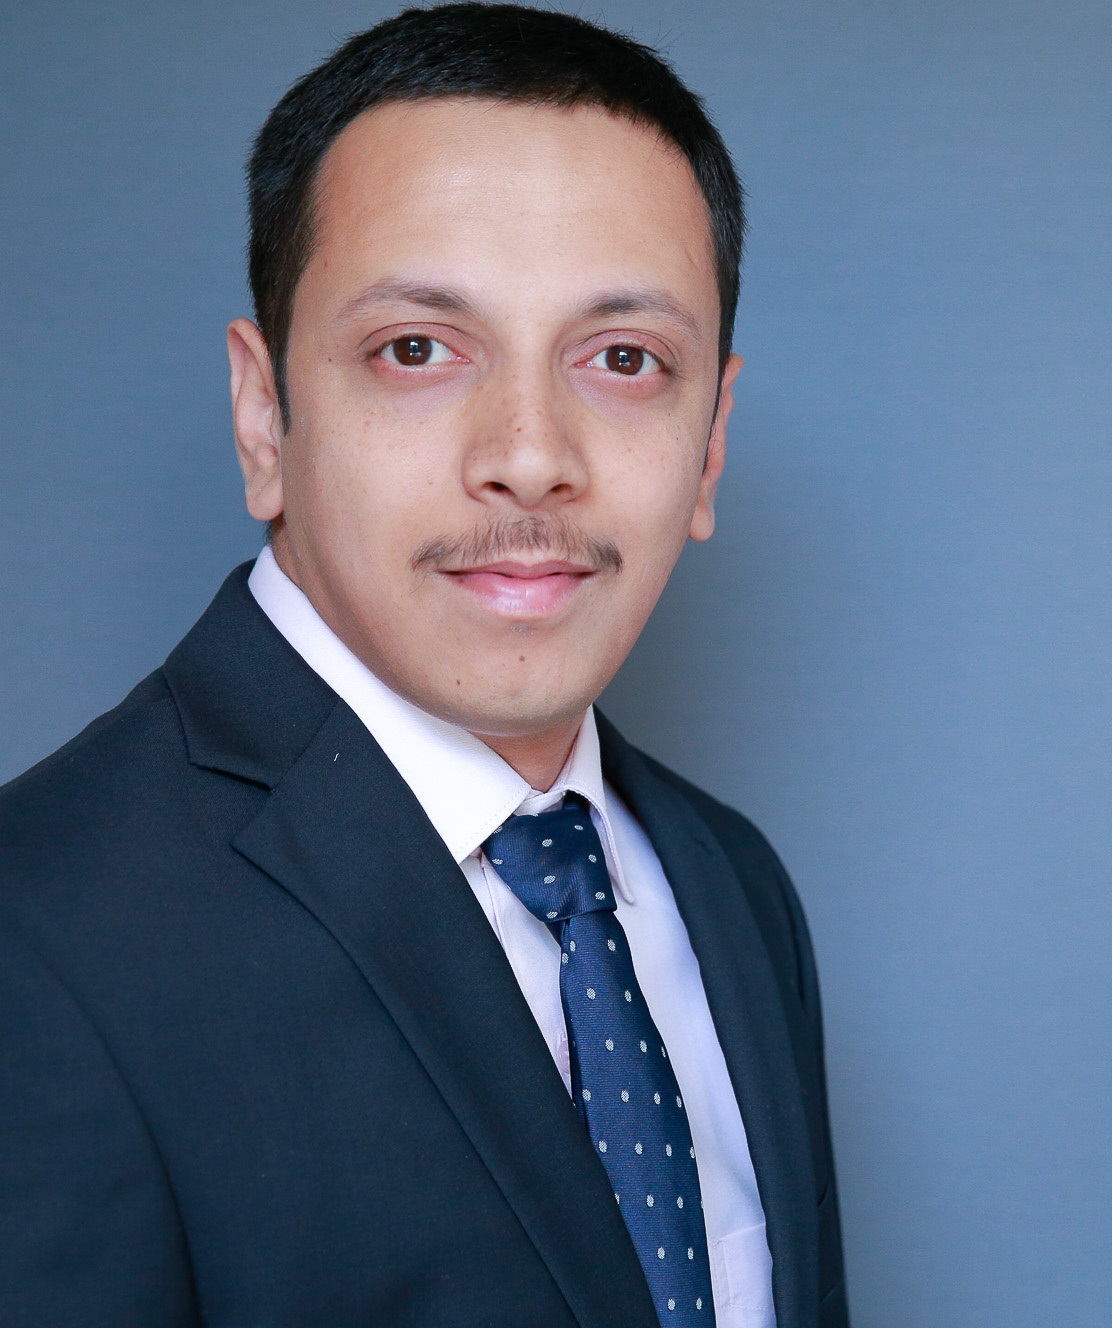
\includegraphics[scale=0.30]{photo}
\par\end{flushright}%
\end{minipage}%
\end{minipage}

\vspace{0.65cm}

\noindent\begin{minipage}[t]{1\columnwidth}%
\textbf{\textcolor{teal}{\large{}Skills :}}{\large \par}

\rule[0.5ex]{1\linewidth}{0.04pt}

\vspace{0.5cm}
%
\end{minipage}

\noindent\begin{minipage}[t]{1\linewidth}%
\begin{itemize}
\item \textbf{\small{}Languages: }{\small{}English (Business fluency), }\textbf{\small{}German
(B2 Level)}{\small \par}
\item \textbf{\small{}Programming}{\small{}: Strong programming skills}\textbf{\small{}
}{\small{}in}\textbf{\small{} R}{\small{}, Python, Javascript, Matlab and LabVIEW. }{\small \par}
\item \textbf{\small{}Visualization \& Reporting :}{\small{} }\textbf{\small{}RShiny}{\small{},
Flask, R-Markdown, \LaTeX and D3.js.}{\small \par}
\item \textbf{\small{}Hands on experience: }{\small{}R, Ensemble learning,
Artificial Neural Networks, Deep Learning.}{\small \par}
\item \textbf{\small{}Agile \& Productivity:}{\small{} SCRUM, JIRA , Confluence,
GIT and SVN.}{\small \par}
\item {\small{}Skills in web-frontend development (HTML5, CSS, PHP, etc.) }{\small \par}
\end{itemize}
%
\end{minipage}
\vspace{0.35cm}

\rule[0.5ex]{1\linewidth}{0.04pt}

\vspace{0.5cm}

\begin{minipage}[t]{0.35\linewidth}%

\section*{\textcolor{teal}{\large{}Education Summary: }}
\begin{itemize}
\item \begin{flushleft}
\textbf{Ph.D. Applied Physics} - University of Saarland (UDS), Saarbr\"uken,
Germany. 
\par\end{flushleft}
\item \begin{flushleft}
\textbf{M.Sc. Theoretical Physics} - Kuvempu University, Karnataka,
India. 
\par\end{flushleft}

\end{itemize}
%
\end{minipage}\hspace{0.25cm}%
\begin{minipage}[t]{0.65\linewidth}%

\section*{\textcolor{teal}{\large{}Resume:}}

I am a Physicist and a Data scientist experienced with advanced Machine
learning algorithms and visual analytics. My interests are in solving complex business challenges by leveraging the data and applying advanced machine learning methods.
Currently, my focus is in  Natural Language Processing or making machines understand and generate human language. For many years I have worked as a researcher in various high-performance research and development environments focused on cutting-edge innovation in science and technology. %
\end{minipage}

\vspace{0.35cm}

\noindent\begin{minipage}[t]{1\columnwidth}%
\textbf{\textcolor{teal}{\large{}Work Experiences:}}{\large \par}

\rule[0.5ex]{1\linewidth}{0.04pt}%
\end{minipage}

\vspace{0.55cm}

\begin{tabular*}{0.8\linewidth}{@{\extracolsep{\fill}}lr}
\begin{minipage}[t]{0.82\linewidth}%
\textbf{\textcolor{black}{Data Scientist and Project Coordinator - Digital Transformation Strategy in Legal and compliance, Stuttgart.}}
\begin{itemize}
\item Working on use cases with state-of-the-art machine learning and NLP techniques.
\item Deep learning.
\item Natural Language Understanding and Natural Language Generation.
\item Topic detection, Topic classification.
\item Building models to extract Semantically similar documents or texts.
\item Developing semantic search tool for news article segregation.
\end{itemize}
%
\end{minipage} & \textbf{\textcolor{black}{\hspace{0.25cm}09/2019- Current}}\tabularnewline
\end{tabular*}


\begin{tabular*}{0.8\linewidth}{@{\extracolsep{\fill}}lr}
\begin{minipage}[t]{0.82\linewidth}%
\textbf{\textcolor{black}{Data Scientist, Daimler Financial Services
(DFS), Stuttgart.}}
\begin{itemize}
\item Built prediction models for CRM Lead conversions and Customer retention.
\begin{itemize}
\item Ensemble prediction models with various machine learning
techniques such as Support Vector Machines and Artificial Neural Network.
\item Developing shiny apps.
\item Worked in Scrum environment to deliver innovative results
under tight timeline constraints and technical difficulties
\end{itemize}
\item \textbf{SpringbokView}: 
\begin{itemize}
\item Created interactive visualization package in R, based on D3.js. it
consists of many advanced visualization types applicable to many scenarios
.Some of the major visualisation functions includes Parallel coordinates,
Association rule mining.
\end{itemize}
\end{itemize}
%
\end{minipage} & \textbf{\textcolor{black}{\hspace{0.25cm}11/2016- 08/2019}}\tabularnewline
\end{tabular*}

\vspace{1cm}

\begin{tabular}{cc}
\begin{minipage}[t]{0.8\linewidth}%
\begin{flushleft}
\textbf{\textcolor{black}{Postdoctoral Researcher, INM - Leibniz Institut
f\"ur neue Materialien, Saarbrucken, Germany.}}
\par\end{flushleft}
\begin{itemize}
\item Measurement and Data Analysis, Data visualization \& Background in
optimization problems.
\item Image processing \& Mathematical modeling in Matlab and Python.
\end{itemize}
%
\end{minipage} & \textbf{\textcolor{black}{\hspace{0.25cm}07/2015- 12/2015}}\tabularnewline
\end{tabular}

\vspace{1cm}

\begin{tabular}{cc}
\begin{minipage}[t]{0.8\linewidth}%
\begin{flushleft}
\textbf{\textcolor{black}{PhD student, INM - Leibniz Institut f\"ur
neue Materialien, Saarbrucken, Germany.}}
\par\end{flushleft}
\begin{itemize}
\item Research into nano mechanical properties of graphitic materials
\item High resolution imaging with Atomic Force Microscope in Ultra High
Vacuum.
\item Image processing \& Mathematical modeling in Matlab and Python.
\item Research publications in very high ranking journals\@.
\end{itemize}
%
\end{minipage} & \textbf{\textcolor{black}{\hspace{0.25cm}07/2011- 06/2015}}\tabularnewline
\end{tabular}

\vspace{1cm}

\noindent\begin{minipage}[t]{1\linewidth}%

\section*{\textcolor{teal}{\large{}Publications:}}

\rule[0.5ex]{1\linewidth}{0.04pt}

\subsection*{\textcolor{black}{\small{}Peer-reviewed publications in high ranking
journals and cited multiple times.}}
\begin{enumerate}
\item \textbf{\small{}Balakrishna, S. G., }{\small{}de Wijn, A. S., \& Bennewitz,
R. (2014). Preferential sliding directions on graphite. Physical Review
B, 89(24), 245440.}{\small \par}
\item {\small{}Klemenz, A., Pastewka, L., }\textbf{\small{}Balakrishna,
S. G.,}{\small{} Caron, A., Bennewitz, R., \& Moseler, M. (2014).
Atomic scale mechanisms of friction reduction and wear protection
by graphene. Nano letters, 14(12), 7145-7152.}{\small \par}
\item {\small{}Chan, N., }\textbf{\small{}Balakrishna, S. G}{\small{}.,
Klemenz, A., Moseler, M., Egberts, P., \& Bennewitz, R. (2017). Contrast
in nanoscale friction between rotational domains of graphene on Pt
(111). Carbon, 113, 132-138.}{\small \par}
\end{enumerate}
%
\end{minipage}
\end{document}
